\section{Simulation Results and Verification}
\label{sec:results-and-verification}

\subsection{Reflection Coefficient and Resonance}

Figure~\ref{fig:s11-result} contains the exact displayed CST marker
\begin{equation}
f_{\mathrm{res}}=0.9186~\text{GHz},\qquad
S_{11,\min}=-22.14379~\text{dB}.
\label{eq:final-s11}
\end{equation}
The corresponding positive return loss is
\begin{equation}
\mathrm{RL}=-S_{11,\mathrm{dB}}=22.14379~\text{dB}.
\label{eq:return-loss}
\end{equation}
This terminology is important: the plotted quantity is the negative dB magnitude of
$S_{11}$, while return loss is conventionally reported as a positive number.

The frequency error is
\begin{equation}
\frac{0.9186-0.915}{0.915}\times100=0.393\%.
\label{eq:frequency-error}
\end{equation}
The marker also implies $|\Gamma|=0.0782$ and a derived VSWR of approximately 1.17,
relative to the configured CST port reference.

\begin{figure}[H]
    \centering
    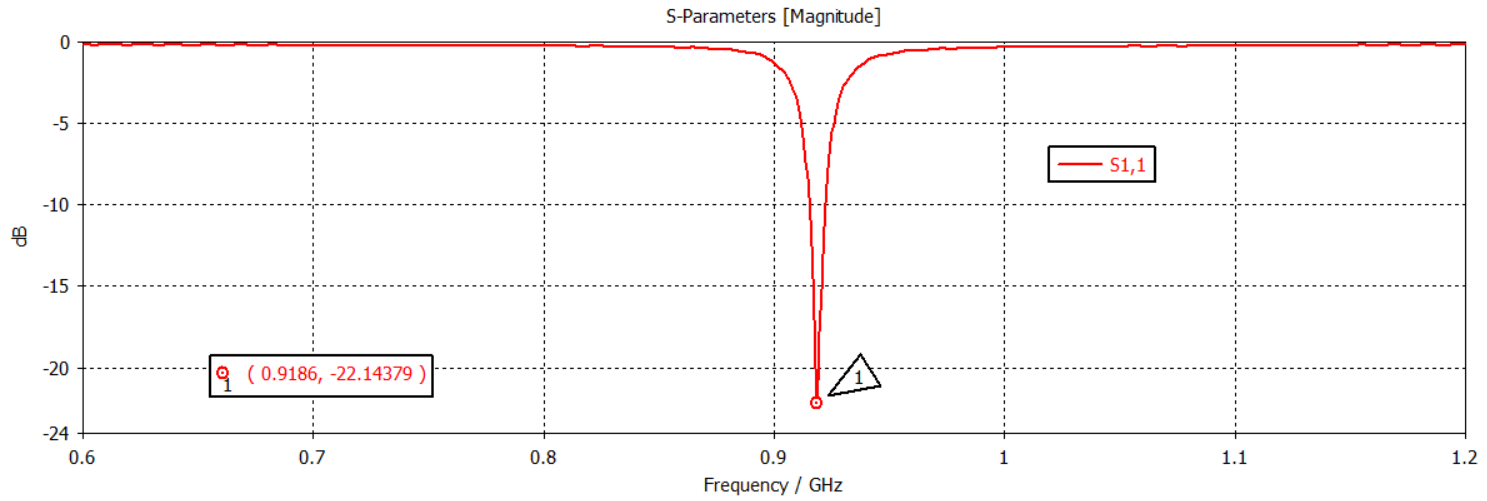
\includegraphics[width=0.94\textwidth]{figures/cst_results/fig_s11_final_915MHz_patch.png}
    \caption{Preserved CST reflection-coefficient plot. The marker identifies the matching minimum at 0.9186~GHz and $S_{11}=-22.14379$~dB.}
    \label{fig:s11-result}
\end{figure}

\begin{table}[H]
\centering
\caption{Final input-match results and derived quantities.}
\label{tab:input-match-results}
\begin{tabular}{@{}lll@{}}
\toprule
\textbf{Quantity} & \textbf{Value} & \textbf{Evidence type} \\
\midrule
Design frequency & 0.915~GHz & Specification \\
Matching-minimum frequency & 0.9186~GHz & Exact displayed marker \\
Minimum $S_{11}$ & -22.14379~dB & Exact displayed marker \\
Positive return loss & 22.14379~dB & Derived from marker \\
Reflection magnitude $|\Gamma|$ & 0.0782 & Derived from marker \\
VSWR & 1.17 & Derived from marker \\
Frequency error & 0.393\% & Derived from marker \\
\bottomrule
\end{tabular}
\end{table}

\subsection{Electric- and Magnetic-Field Evidence}

The preserved field monitors were evaluated at 0.915~GHz. Figures
\ref{fig:efield-result} and \ref{fig:hfield-result} show concentration around the patch,
inset, and feed region. These images support resonant excitation qualitatively, but no
raw field export is available for independent quantitative post-processing.

\begin{figure}[H]
    \centering
    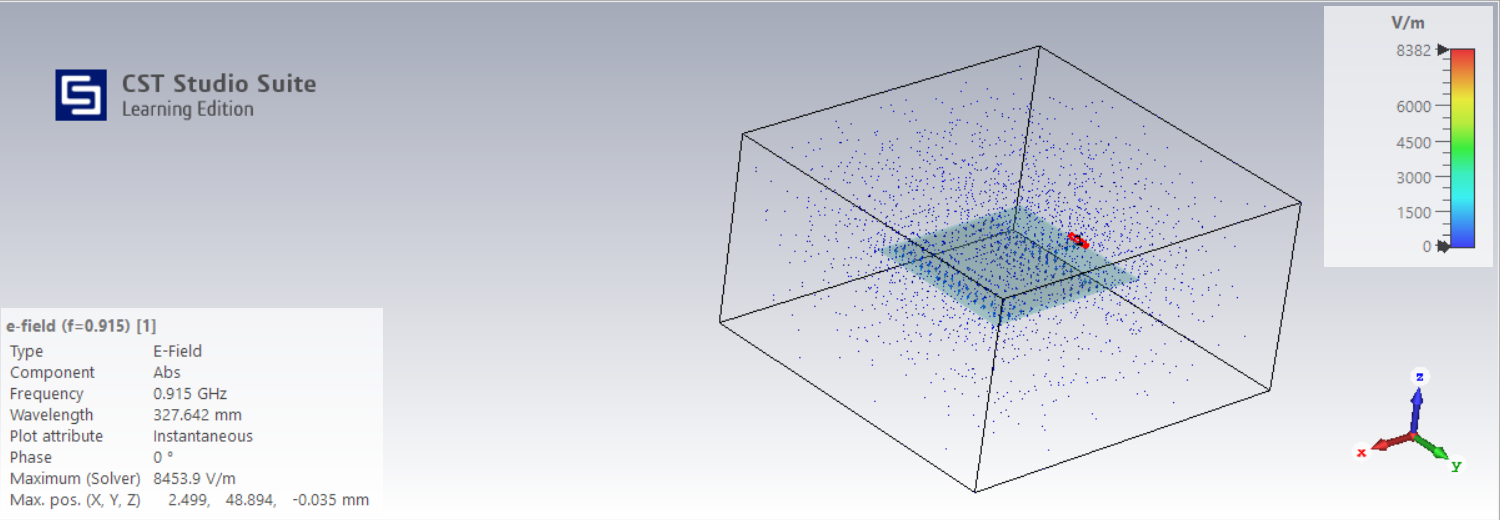
\includegraphics[width=0.94\textwidth]{figures/cst_results/fig_efield_915MHz.png}
    \caption{Simulated electric-field distribution at 0.915~GHz.}
    \label{fig:efield-result}
\end{figure}

\begin{figure}[H]
    \centering
    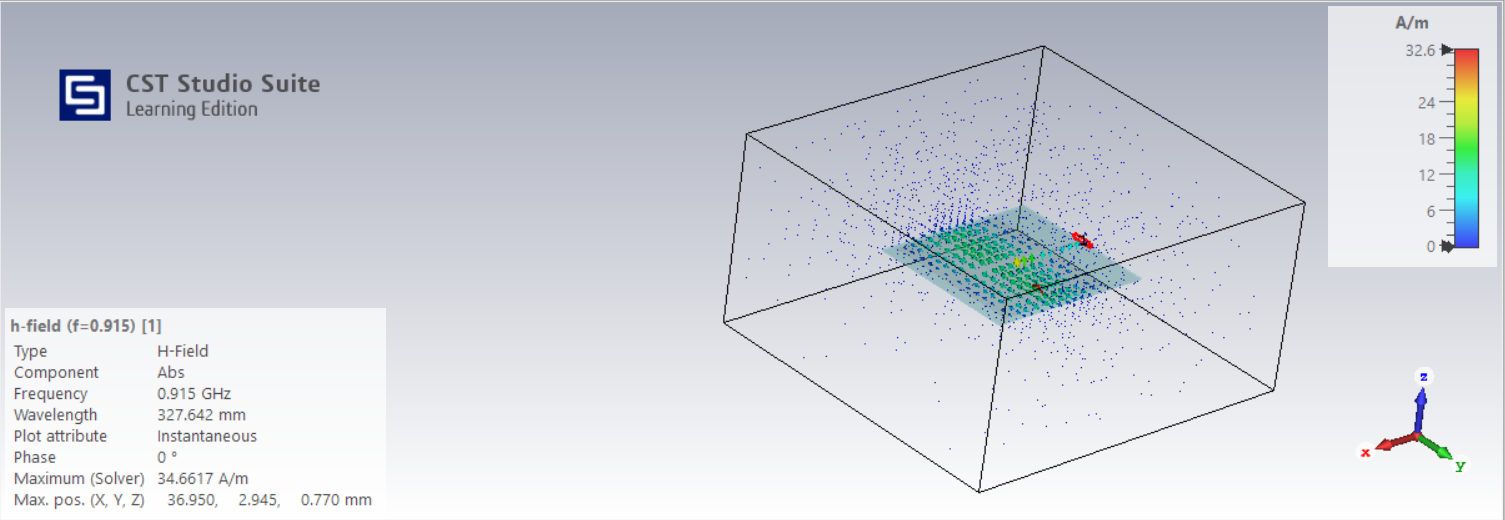
\includegraphics[width=0.94\textwidth]{figures/cst_results/fig_hfield_915MHz.png}
    \caption{Simulated magnetic-field distribution at 0.915~GHz.}
    \label{fig:hfield-result}
\end{figure}

\subsection{Three-Dimensional Far Field}

The CST 3D plot in Fig.~\ref{fig:farfield-3d} displays a broadside main lobe and a peak
directivity of 7.01~dBi at 0.915~GHz. The information panel also displays radiation
efficiency of 0.03436~dB and total efficiency of -0.4787~dB. Because the radiation
efficiency is slightly positive in dB, it corresponds to a value marginally above
100\% and is treated as a numerical-display anomaly rather than a validated efficiency
claim. The total-efficiency display is retained as supporting evidence but is not used as
a principal performance KPI without convergence and raw data.

\begin{figure}[H]
    \centering
    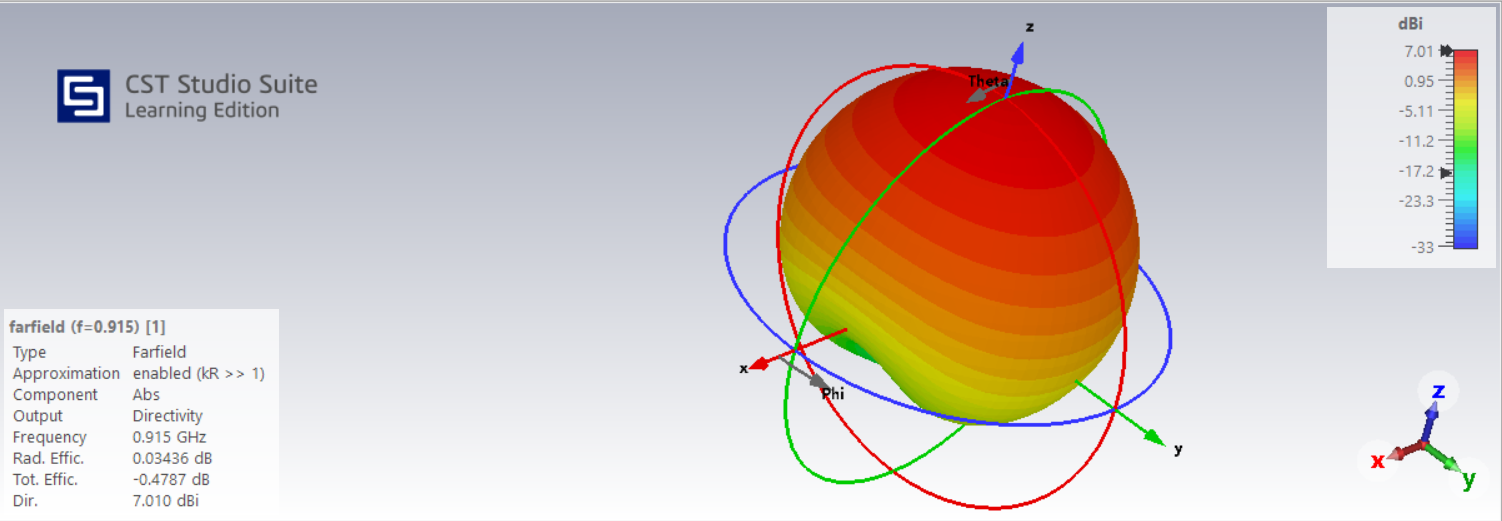
\includegraphics[width=0.95\textwidth]{figures/cst_results/fig_3d_radiation_pattern_915MHz.png}
    \caption{CST 3D far-field directivity at 0.915~GHz. The displayed peak is 7.01~dBi.}
    \label{fig:farfield-3d}
\end{figure}

\subsection{Principal-Plane Radiation Patterns}

Figures \ref{fig:phi0-pattern} and \ref{fig:phi90-pattern} show the two documented
principal-plane cuts. Both support broadside radiation. The $\phi=0^\circ$ cut includes
a displayed sidelobe level of -19.2~dB; no corresponding sidelobe value is shown in the
$\phi=90^\circ$ screenshot.

\begin{figure}[H]
    \centering
    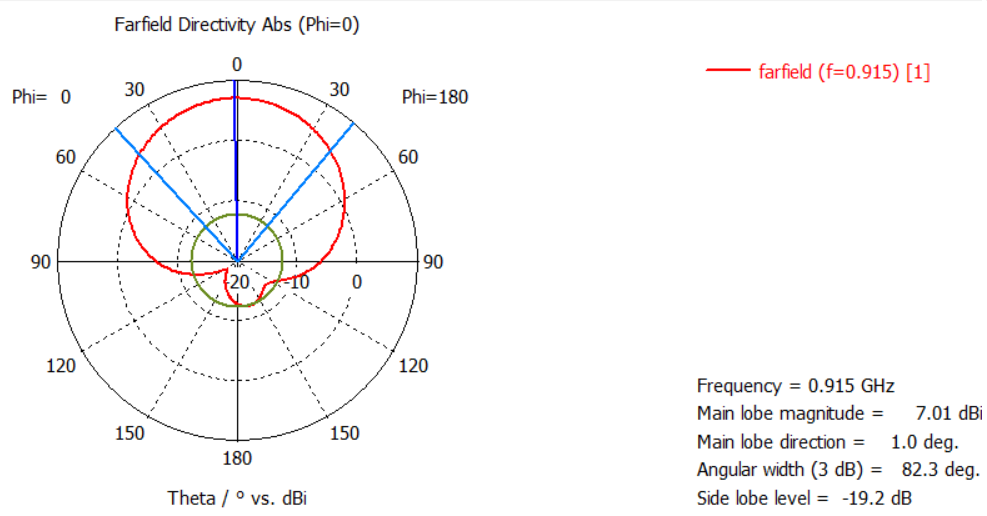
\includegraphics[width=0.78\textwidth]{figures/cst_results/fig_2d_polar_pattern_phi0_915MHz.png}
    \caption{CST principal-plane directivity pattern at 0.915~GHz for $\phi=0^\circ$.}
    \label{fig:phi0-pattern}
\end{figure}

\begin{figure}[H]
    \centering
    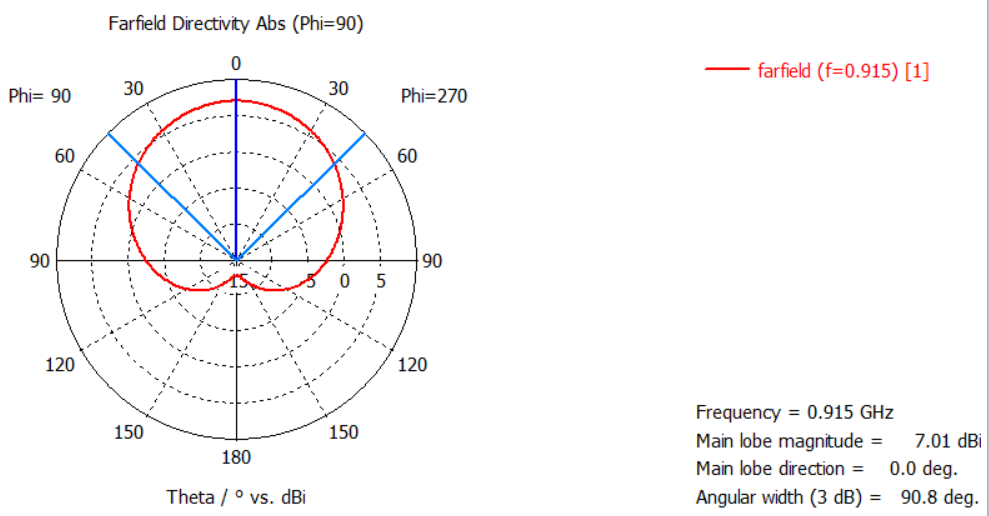
\includegraphics[width=0.78\textwidth]{figures/cst_results/fig_2d_polar_pattern_phi90_915MHz.png}
    \caption{CST principal-plane directivity pattern at 0.915~GHz for $\phi=90^\circ$.}
    \label{fig:phi90-pattern}
\end{figure}

\begin{table}[H]
\centering
\caption{Displayed principal-plane far-field quantities at 0.915~GHz.}
\label{tab:principal-plane-results}
\begin{tabular}{@{}lllll@{}}
\toprule
\textbf{Cut} & \textbf{Peak} & \textbf{Direction} & \textbf{3-dB width} & \textbf{Displayed SLL} \\
\midrule
$\phi=0^\circ$ & 7.01~dBi & 1.0$^\circ$ & 82.3$^\circ$ & -19.2~dB \\
$\phi=90^\circ$ & 7.01~dBi & 0.0$^\circ$ & 90.8$^\circ$ & Not displayed \\
\bottomrule
\end{tabular}
\end{table}
